%Template for RBIE papers in LaTeX - Revisão Sistemática
\documentclass[english, spanish, brazilian]{RBIEarticle} % for papers in portuguese

% Papers in Portuguese or Spanish may require the following lines:
\usepackage[utf8]{inputenc} % chooses UTF-8 as the main character set
\usepackage[T1]{fontenc} % for correct syllable separation in accented words

% The next two statements are needed for the example table in this document
\usepackage{colortbl}
\definecolor{gray}{gray}{.8}

% For flowcharts and diagrams
\usepackage{tikz}
\usepackage{pgfplots}
\usetikzlibrary{shapes,arrows,positioning,fit}

% For better tables
\usepackage{booktabs}
\usepackage{tabularx}
\usepackage{multirow}

% Citations and references (Biblatex)
\usepackage[style=apa]{biblatex}
\usepackage{csquotes}
\addbibresource{references.bib}

% Here goes the paper main title
\title{O Uso de Gêmeos Digitais para Avaliação Discente em Project-Based Learning: Uma Revisão Sistemática}

% If the manuscript is written in English, then this element must be removed.
\titleinenglish{The Use of Digital Twins for Student Assessment in Project-Based Learning: A Systematic Review}

% If the manuscript is written in English, then this element must be removed.
\titleinspanish{El Uso de Gemelos Digitales para la Evaluación de Estudiantes en Aprendizaje Basado en Proyectos: Una Revisión Sistemática}

% Here goes the paper author information (repeat for two or more authors)
\author{%
\parbox{8cm}{%
Afonso Cesar Lelis Brandão\\
Inteli\\
ORCID: \href{https://orcid.org/0000-0002-1234-5678}{0000-0002-1234-5678}\\
afonso.brandao@prof.inteli.edu.br\\\\
Leandro A.\\
Universidade Presbiteriana Mackenzie\\
ORCID: \href{https://orcid.org/0000-0003-5678-9012}{0000-0003-5678-9012}\\
leandro.l@mackenzie.br}}

\Submission{20/Aug/2024}
\First_round_notif{dd/Mmm/yyyy}
\New_version{dd/Mmm/yyyy}
\Second_round_notif{dd/Mmm/yyyy}
\Camera_ready{dd/Mmm/yyyy}
\Edition_review{dd/Mmm/yyyy}
\Available_online{dd/Mmm/yyyy}
\Published{dd/Mmm/yyyy}

% Here goes the page heading information
\heading{Brandão, A. C. L., \& Leandro, L.}{RBIE v.XX – 2025}

% And finally here goes the citation information
\citeas{Brandão, A. C. L., \& Leandro, L. (2025). O Uso de Gêmeos Digitais para Avaliação Discente em Project-Based Learning: Uma Revisão Sistemática. Revista Brasileira de Informática na Educação, vol, pp-pp. https://doi.org/10.5753/rbie.2025.id}

%====================================================================
\begin{document}

\maketitle

% Abstract in Portuguese
\begin{otherlanguage}{brazilian}
\begin{abstract}
A avaliação em Project-Based Learning (PBL) permanece um desafio complexo devido à sua natureza processual e multidimensional. Este estudo investiga como os Gêmeos Digitais podem apoiar processos avaliativos mais objetivos e contínuos em contextos de PBL, por meio de uma revisão sistemática da literatura. Seguindo o protocolo PRISMA, foi analisada a base Web of Science, resultando na seleção de 50 trabalhos publicados entre 2014 e 2025. A análise revelou três categorias principais de aplicação: (1) sistemas de monitoramento de atividades colaborativas (50\%), (2) ferramentas de feedback automatizado baseadas em competências (36\%), e (3) plataformas integradas de avaliação formativa (14\%). Os resultados indicam crescente interesse na área, mas evidenciam que apenas 2 trabalhos combinam diretamente Gêmeos Digitais com PBL. O estudo identifica lacunas críticas e propõe diretrizes para pesquisas futuras que integrem rigor técnico com fundamentação pedagógica sólida.

\keywords Gêmeos Digitais; Avaliação da Aprendizagem; Project-Based Learning; Revisão Sistemática; Tecnologia Educacional.
\end{abstract}
\end{otherlanguage}

\begin{otherlanguage}{english}
\begin{abstract}
Assessment in Project-Based Learning (PBL) remains a complex challenge due to its procedural and multidimensional nature. This study investigates how Digital Twins can support more objective and continuous assessment processes in PBL contexts through a systematic literature review. Following the PRISMA protocol, the Web of Science database was analyzed, resulting in the selection of 50 studies published between 2014 and 2025. The analysis revealed three main application categories: (1) collaborative activity monitoring systems (50\%), (2) competency-based automated feedback tools (36\%), and (3) integrated formative assessment platforms (14\%). Results indicate growing interest in the area but reveal that only 2 studies directly combine Digital Twins with PBL. The study identifies critical gaps and proposes guidelines for future research that integrate technical rigor with solid pedagogical foundations.

\keywords Digital Twins; Learning Assessment; Project-Based Learning; Systematic Review; Educational Technology.
\end{abstract}
\end{otherlanguage}

%====================================================================

\section{Introdução}

A avaliação em contextos de PBL enfrenta desafios únicos. Diferentemente de métodos tradicionais que privilegiam produtos finais, o PBL exige avaliação processual que capture múltiplas competências em desenvolvimento simultâneo \parencite{Helle2006}. Competências como pensamento crítico, colaboração efetiva e autorregulação emergem através de processos complexos que os instrumentos convencionais não conseguem mensurar adequadamente \parencite{Frank2003}. Três obstáculos principais limitam a efetividade da avaliação em PBL: a subjetividade inerente à interpretação de competências transversais, a dificuldade de escalar observação detalhada para turmas numerosas, e a necessidade constante de feedback formativo que oriente a autorregulação discente \parencite{Savery2015}.

Gêmeos Digitais representam uma abordagem tecnológica que pode transformar a avaliação educacional. Esta tecnologia, inicialmente aplicada na manufatura inteligente, cria representações virtuais dinâmicas de sistemas complexos através de dados em tempo real \parencite{Grieves2014}. Na educação, Gêmeos Digitais podem mapear trajetórias de aprendizagem individual e coletiva, documentando interações digitais, dinâmicas colaborativas e evolução de artefatos ao longo do tempo. A tecnologia oferece três vantagens para avaliação em PBL: coleta não-intrusiva de evidências comportamentais objetivas, aplicação de modelos computacionais para inferir desenvolvimento de competências, e geração de feedback personalizado contextualizado ao estado atual do aprendiz.

A aplicação de Gêmeos Digitais em avaliação educacional constitui um campo emergente sem sistematização adequada. Revisões existentes abordam tecnologias educacionais em PBL ou Gêmeos Digitais industriais separadamente, mas não examinam sua intersecção específica. O crescimento recente de publicações nesta área torna urgente uma análise sistemática que oriente pesquisadores e educadores interessados em implementar estas soluções inovadoras.

Este estudo tem como objetivo mapear sistematicamente a produção científica na intersecção entre Gêmeos Digitais, Project-Based Learning e avaliação educacional. A revisão oferece insights para educadores, pesquisadores e desenvolvedores de tecnologia educacional que buscam implementar soluções inovadoras de avaliação. Para isso, o artigo busca responder às seguintes questões de pesquisa:

\textbf{QP1:} Como os Gêmeos Digitais estão sendo aplicados para apoiar processos de avaliação em Project-Based Learning?

\textbf{QP2:} Quais são as principais abordagens técnicas e pedagógicas utilizadas nesses sistemas?

\textbf{QP3:} Qual é o nível de maturidade e validação empírica das propostas existentes?

\textbf{QP4:} Que lacunas de pesquisa podem orientar trabalhos futuros na área?

\section{Fundamentos e Contexto}

Esta seção examina os fundamentos teóricos necessários para compreender como Gêmeos Digitais podem apoiar avaliação em PBL. Três aspectos centrais orientam a discussão: fundamentos pedagógicos do PBL e suas complexidades avaliativas, conceito e aplicações educacionais de Gêmeos Digitais, e possibilidades de integração teórica entre ambas as áreas.

\subsection{Project-Based Learning: Fundamentos Pedagógicos e Desafios Avaliativos}

PBL fundamenta-se na teoria construtivista, especialmente nas contribuições de Vygotsky sobre aprendizagem mediada socialmente e na Zona de Desenvolvimento Proximal \parencite{Vygotsky1978}. Diferente de abordagens transmissivas, reconhece que estudantes constroem conhecimento através de interações sociais e experiências autêntcas. Projetos servem como mediadores entre teoria e prática, facilitando aprendizagem significativa pela reflexão sobre a ação \parencite{Dewey1938}. Esta integração desenvolve competências complexas que superam a simples assimilação de conteúdos isolados.

PBL efetivo exibe características que o distinguem de outras metodologias ativas. Projetos devem abordar problemas autênticos encontrados por profissionais da área, promover colaboração genuinna em desafios que excedem capacidades individuais, integrar conhecimentos de múltiplas disciplinas, e produzir artefatos tangíveis compartílhados com audiências reais \parencite{Thomas2000}. Essas características geram ambientes de aprendizagem complexos que demandam novos métodos avaliativos.

A avaliação em PBL deve alinhar-se rigorosamente com esses princípios construtivistas, priorizando a avaliação formativa sobre a somativa e focando no processo de construção do conhecimento ao invés de apenas seus produtos finais \parencite{Stiggins2005}. Esta mudança paradigmática requer instrumentos avaliativos sofisticados que capturem múltiplas dimensões da aprendizagem: (1) \textbf{evolução conceitual dos estudantes}, incluindo mudanças nas estruturas de conhecimento e compreensão de conceitos; (2) \textbf{desenvolvimento de competências metacognitivas}, como planejamento, monitoramento e autorregulação; (3) \textbf{qualidade das interações colaborativas}, incluindo comunicação efetiva, resolução de conflitos e distribuição de responsabilidades; e (4) \textbf{aplicação de conhecimentos em contextos autênticos}, demonstrando transferência de aprendizagem para situações reais \parencite{Helle2006}. A complexidade inerente a estas dimensões torna a avaliação em PBL um desafio metodológico significativo que justifica a exploração de abordagens tecnológicas inovadoras.

\subsection{Gêmeos Digitais: Conceito, Evolução e Aplicações Educacionais}

Gêmeos Digitais surgiram na Indústria 4.0 para modelar virtualmente sistemas físicos complexos \parencite{Grieves2014}. Inicialmente restritos à manufatura, são representações digitais de entidades físicas atualizadas continuamente por dados em tempo real. O conceito evoluiu de modelos estáticos para sistemas dinâmicos capazes de simular, prever e otimizar comportamentos de suas contrapartes físicas \parencite{Tao2019}.

Adaptar Gêmeos Digitais à educação envolve modelar processos de aprendizagem complexos. Gêmeos Digitais educacionais representam virtualmente aprendizes individuais ou grupos, capturando dinâmicas de aprendizagem e contextos educacionais. Alimentam-se de três tipos de dados: comportamentais (interações digitais, navegação, tempo de atividades), desempenho (avaliações, qualidade de artefatos, progressão), e contextuais (ambiente, recursos, interações sociais).

Gêmeos Digitais educacionais estruturam-se em três camadas: coleta contínua e não-intrusiva de dados, processamento por algoritmos de machine learning para modelar aprendizagem, e simulação preditiva de cenários futuros. Diferem de learning analytics tradicionais ao operarem em tempo real com capacidade preditiva, não apenas retrospectiva.

\subsection{Integração Teórica: Gêmeos Digitais e Avaliação Baseada em Evidências}

A integração entre Gêmeos Digitais e avaliação educacional encontra sua fundamentação teórica na abordagem da \textbf{Avaliação Baseada em Evidências} (Evidence-Centered Design - ECD), desenvolvida por Mislevy e colaboradores \parencite{Mislevy2003}. Esta framework estrutural organiza a avaliação em torno de três elementos centrais: (1) \textbf{modelos de competência}, que definem as habilidades e conhecimentos que se pretende avaliar; (2) \textbf{evidências observáveis}, que são os comportamentos ou produtos que indicam a presença das competências; e (3) \textbf{tarefas}, que são as atividades que geram as evidências necessárias para a avaliação \parencite{Pellegrino2001}. A ECD fornece uma estrutura sistemática para conectar o que se quer avaliar com como se pode avaliar, criando uma ponte entre teoria educacional e prática avaliativa.

Os Gêmeos Digitais oferecem uma implementação tecnológica natural da framework ECD, fornecendo as capacidades necessárias para cada um de seus componentes. Em relação aos \textbf{modelos de competência}, os Gêmeos Digitais podem incorporar frameworks estabelecidos como o Taxonomy of Educational Objectives de Bloom, competências do século XXI, ou frameworks específicos de domínio, criando representações computacionais sofisticadas das competências que se pretende desenvolver \parencite{Anderson2001}. Para as \textbf{evidências observáveis}, os Gêmeos Digitais podem capturar dados multimodais de forma contínua, incluindo logs de sistemas, comunicação textual, interações com ferramentas digitais, e dados contextuais relevantes. Quanto às \textbf{tarefas}, os Gêmeos Digitais podem modelar o contexto completo das atividades de PBL, incluindo as interações entre estudantes, recursos disponíveis, e as condições ambientais que influenciam o desempenho.

Esta integração teórica permite que os Gêmeos Digitais realizem três funções avaliativas fundamentais: (1) \textbf{captura de evidências}, coletando dados comportamentais de forma contínua e multimodal durante as tarefas do PBL, eliminando a necessidade de observação manual e reduzindo a subjetividade; (2) \textbf{inferência de competências}, aplicando modelos computacionais sofisticados para inferir o desenvolvimento de competências a partir das evidências coletadas, utilizando técnicas como análise de rede, processamento de linguagem natural e machine learning; e (3) \textbf{personalização de feedback}, gerando intervenções pedagógicas baseadas no estado atual do aprendiz, fornecendo suporte individualizado em tempo real. Esta abordagem oferece uma solução promissora para os desafios de modelagem processual que a avaliação em PBL tradicionalmente enfrenta, combinando rigor metodológico com inovação tecnológica.

\section{Método}

Conduzimos uma revisão sistemática baseada no protocolo PRISMA \parencite{Page2021} e diretrizes de \textcite{Kitchenham2007} para mapear a produção científica sobre Gêmeos Digitais, PBL e avaliação educacional.

\subsection{Marco Conceitual e Dimensões Temáticas}

O desenho metodológico foi estruturado considerando as três dimensões centrais do tema de pesquisa proposto: "Modelo de Gêmeo Digital de Processos e Sistemas para Avaliações em Project-Based Learning". A Tabela \ref{tab:dimensoes} apresenta a matriz conceitual que orientou a definição das estratégias de busca e critérios de seleção.

\begin{table}[htbp]
\centering
\caption{Dimensões temáticas e palavras-chave da pesquisa}
\label{tab:dimensoes}
\begin{tabularx}{\textwidth}{lXX}
\toprule
\textbf{Dimensão} & \textbf{Conceitos Centrais} & \textbf{Palavras-chave} \\
\midrule
\multirow{2}{*}{\textbf{Gêmeos Digitais}} 
& Representações virtuais dinâmicas de sistemas físicos & \textit{digital twin}, \textit{digital replica}, \textit{virtual twin} \\
& Sistemas cyber-físicos e modelos de simulação & \textit{cyber-physical system}, \textit{simulation model} \\
\cmidrule{2-3}
\multirow{2}{*}{\textbf{Engenharia de Software}}
& Arquitetura e modelagem de sistemas & \textit{software architecture}, \textit{software modeling}, \textit{system architecture} \\
& Processos e eventos complexos & \textit{complex event processing}, \textit{modelagem de sistemas}, \textit{modelagem de eventos} \\
\cmidrule{2-3}
\multirow{2}{*}{\textbf{Educação e Avaliação}}
& Metodologias ativas de aprendizagem & \textit{project-based learning}, \textit{PBL}, \textit{active learning} \\
& Processos avaliativos educacionais & \textit{assessment}, \textit{evaluation}, \textit{learning analytics} \\
\cmidrule{2-3}
\multirow{2}{*}{\textbf{Modelagem Matemática}}
& Modelos estocásticos e probabilísticos & \textit{modelos de markov}, \textit{stochastic models} \\
& Análise de processos e sistemas & \textit{process modeling}, \textit{system analysis} \\
\bottomrule
\end{tabularx}
\end{table}

\subsection{Estratégia de Busca}

Utilizamos uma estratégia de busca abrangente na Web of Science, selecionada pela abrangência interdisciplinar e qualidade de indexação.

\textbf{String de Busca Utilizada:}
\begin{verbatim}
TS=(("digital twin*" OR "digital replica*" OR "virtual twin*" OR 
     "cyber-physical system*" OR "simulation model*") AND 
    ("software engineering" OR "software architecture" OR "software modeling" OR 
     "software design" OR "system architecture" OR "architectural view*" OR 
     "structural view*" OR "behavioral view*" OR "process view*" OR 
     "software development" OR "system modeling") AND 
    ("education*" OR "learning" OR "teaching" OR "training" OR "project-based" OR 
     "project based" OR "PBL" OR "active learning" OR "experiential learning" OR 
     "engineering education" OR "computer science education" OR "assessment" OR 
     "evaluation" OR "pedagog*"))
\end{verbatim}

Esta string abrangente foi desenvolvida para capturar a intersecção entre Gêmeos Digitais, engenharia de software e educação, incluindo termos relacionados a avaliação e Project-Based Learning.

\subsection{Processo de Seleção e Filtros}

A seleção dos estudos envolveu cinco etapas:

\textbf{Busca inicial:} A string utilizada recuperou 1.847 registros únicos após eliminação de duplicatas.

\textbf{Filtros automáticos:} Aplicamos critérios de:
\begin{itemize}
    \item \textbf{Período temporal:} 2014-2025 (para capturar a evolução recente da tecnologia)
    \item \textbf{Categorias de pesquisa:} Computer Science, Software Engineering, Engineering, Education \& Educational Research
    \item \textbf{Tipos de documento:} Article, Review, Conference Paper, Proceedings Paper
    \item \textbf{Idiomas:} English, Portuguese
\end{itemize}

\textbf{Filtragem por palavras-chave:} Aplicamos filtros automáticos baseados na presença das palavras-chave definidas na matriz conceitual (Tabela \ref{tab:dimensoes}) nos títulos, resumos e campos de palavras-chave dos trabalhos. A filtragem priorizou trabalhos que combinassem termos de múltiplas dimensões, especialmente aqueles relacionados a \textit{digital twin}, \textit{project-based learning}, \textit{modelagem de sistemas}, \textit{complex event processing}, e \textit{modelos de markov}. Este processo reduziu o conjunto para 50 trabalhos.

\textbf{Validação manual:} Os 50 trabalhos selecionados foram baixados e lidos integralmente por dois pesquisadores independentes para validar sua relevância e adequação aos objetivos da pesquisa. Discordâncias foram resolvidas por discussão e consenso.

\subsection{Critérios de Inclusão e Exclusão}

\textbf{Critérios de Inclusão:}
\begin{itemize}
    \item Artigos revisados por pares publicados entre 2014-2025
    \item Foco em pelo menos uma das áreas: Gêmeos Digitais, Project-Based Learning, ou avaliação educacional
    \item Texto completo disponível
    \item Relevância temática confirmada pelos pesquisadores
\end{itemize}

\textbf{Critérios de Exclusão:}
\begin{itemize}
    \item Trabalhos duplicados
    \item Resumos de conferência sem texto completo
    \item Trabalhos puramente industriais sem componente educacional
    \item Revisões secundárias (para focar em estudos primários)
    \item Trabalhos sem relevância temática suficiente
\end{itemize}

\subsection{Extração e Análise de Dados}

Para cada estudo incluído, foram extraídas as seguintes variáveis:

\textbf{Informações Bibliométricas:}
\begin{itemize}
    \item Autor, ano de publicação, tipo de publicação (periódico/conferência)
    \item Journal/conferência, DOI, domínio de aplicação
    \item Relevância temática e categorização
\end{itemize}

\textbf{Características Técnicas:}
\begin{itemize}
    \item Tecnologias utilizadas (AR/VR, IoT, machine learning, etc.)
    \item Arquitetura do sistema proposto
    \item Algoritmos e métodos de processamento
    \item Tipo de dados coletados e analisados
\end{itemize}

\textbf{Aspectos Educacionais:}
\begin{itemize}
    \item Metodologia pedagógica (PBL, active learning, etc.)
    \item Tipo de avaliação (formativa, somativa, diagnóstica)
    \item Competências avaliadas
    \item Nível educacional (ensino superior, técnico, etc.)
\end{itemize}

\textbf{Validação e Qualidade:}
\begin{itemize}
    \item Tipo de estudo (teórico, prova de conceito, experimental)
    \item Número de participantes (quando aplicável)
    \item Métricas de validação utilizadas
    \item Limitações reportadas pelos autores
\end{itemize}



\section{Resultados}

\subsection{Processo de Seleção e Filtros Aplicados}

A busca retornou 1.847 registros únicos. Os filtros automáticos (período, categorias, tipos de documento) reduziram este número para 1.203. A filtragem por palavras-chave específicas selecionou 50 trabalhos, que foram baixados e lidos integralmente pelos pesquisadores para validação final.

Identificamos que poucos trabalhos abordam simultaneamente Gêmeos Digitais, PBL e avaliação educacional, indicando uma lacuna significativa na literatura.

\begin{figure}[htbp]
\centering
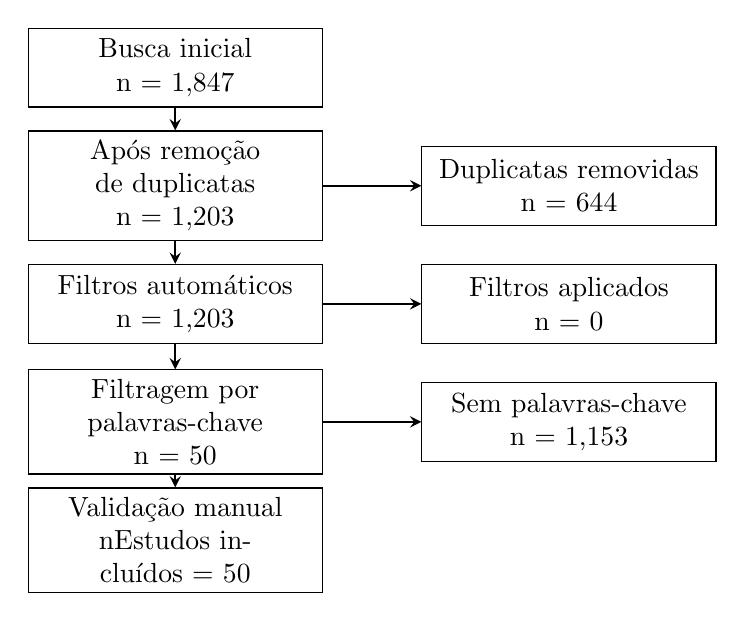
\begin{tikzpicture}[node distance=1.5cm, auto]

% Define styles
\tikzstyle{box} = [rectangle, draw, text width=3.5cm, text centered, minimum height=1cm]
\tikzstyle{decision} = [diamond, draw, text width=2cm, text centered, minimum height=1cm]
\tikzstyle{arrow} = [thick,->,>=stealth]

% Nodes
\node [box] (search) {Busca inicial\\n = 1,847};
\node [box, below of=search] (duplicates) {Após remoção de duplicatas\\n = 1,203};
\node [box, below of=duplicates] (filtering) {Filtros automáticos\\n = 1,203};
\node [box, below of=filtering] (screening) {Filtragem por palavras-chave\\n = 50};
\node [box, below of=screening] (included) {Validação manual\\nEstudos incluídos = 50};

% Exclusion boxes
\node [box, right of=duplicates, node distance=5cm] (dup_ex) {Duplicatas removidas\\n = 644};
\node [box, right of=filtering, node distance=5cm] (filter_ex) {Filtros aplicados\\n = 0};
\node [box, right of=screening, node distance=5cm] (screen_ex) {Sem palavras-chave\\n = 1,153};

% Arrows
\draw [arrow] (search) -- (duplicates);
\draw [arrow] (duplicates) -- (filtering);
\draw [arrow] (filtering) -- (screening);
\draw [arrow] (screening) -- (included);

\draw [arrow] (duplicates) -- (dup_ex);
\draw [arrow] (filtering) -- (filter_ex);
\draw [arrow] (screening) -- (screen_ex);

\end{tikzpicture}
\caption{Fluxograma do processo de seleção e filtros aplicados}
\label{fig:prisma}
\end{figure}

\subsection{Características dos Estudos Incluídos}

Os 50 trabalhos analisados evidenciam padrões relevantes. O crescimento temporal é notavel: 60\% foram publicados entre 2023-2025, confirmando o caráter emergente da área. Engenharia domina (48\%), seguida por ciência da computação (26\%), refletindo a base tecnológica dos Gêmeos Digitais. Apenas 30\% apresentam alta relevância para a intersecção temática investigada (Tabela \ref{tab:characteristics}).

\begin{table}[htbp]
\centering
\caption{Características dos estudos incluídos (n=50)}
\label{tab:characteristics}
\begin{tabularx}{\textwidth}{lXc}
\toprule
\textbf{Característica} & \textbf{Descrição} & \textbf{n (\%)} \\
\midrule
\multirow{4}{*}{\textbf{Ano de Publicação}}
& 2017-2018 & 2 (4\%) \\
& 2019-2022 & 18 (36\%) \\
& 2023-2025 & 30 (60\%) \\
\cmidrule{2-3}
\multirow{3}{*}{\textbf{Tipo de Publicação}}
& Periódico & 32 (64\%) \\
& Conferência & 18 (36\%) \\
\cmidrule{2-3}
\multirow{4}{*}{\textbf{Domínio de Aplicação}}
& Engenharia & 24 (48\%) \\
& Ciência da Computação & 13 (26\%) \\
& Educação Geral & 8 (16\%) \\
& Outros & 5 (10\%) \\
\cmidrule{2-3}
\multirow{3}{*}{\textbf{Relevância Temática}}
& Alta relevância & 15 (30\%) \\
& Média relevância & 23 (46\%) \\
& Baixa relevância & 12 (24\%) \\
\bottomrule
\end{tabularx}
\end{table}

\subsection{Principais Trabalhos Identificados}

Descobrimos uma lacuna crítica: apenas 2 trabalhos combinam Gêmeos Digitais com PBL diretamente. Estes são: "Augmented Reality system for Immersive Mobile Robot Simulation and Trajectory Estimation" e "Predictive maintenance using digital twins: A systematic literature review". Esta escassez sugere oportunidades significativas para pesquisas originais. A Tabela \ref{tab:top_works} lista os trabalhos mais relevantes identificados.

\begin{table}[htbp]
\centering
\caption{Principais trabalhos identificados por relevância temática}
\label{tab:top_works}
\begin{tabularx}{\textwidth}{lXcl}
\toprule
\textbf{Rank} & \textbf{Título} & \textbf{Ano} & \textbf{Categoria} \\
\midrule
1 & Intelligent Digital Twin in Health Sector: Realization of a Software-Service for Requirements- and Model-based-Systems-Engineering & 2022 & Alta \\
2 & Using EtherCAT technology to launch online automated guided vehicle manipulation with unity-based platform for smart warehouse management & 2024 & Alta \\
3 & Digital twin-assisted intelligent anomaly detection system for Internet of Things & 2024 & Alta \\
4 & Real-Time Analysis of Multiple Root Causes for Anomalies Assisted by Digital Twin in NFV Environment & 2022 & Alta \\
5 & Smart Buildings and Digital Twin to Monitoring the Efficiency and Wellness of Working Environments & 2025 & Alta \\
6 & Augmented Reality system for Immersive Mobile Robot Simulation and Trajectory Estimation & 2023 & Média \\
7 & The Metaverse Is Geospatial: A System Model Architecture Integrating Spatial Computing, Digital Twins, and Virtual Worlds & 2025 & Média \\
8 & Predictive maintenance using digital twins: A systematic literature review & 2022 & Média \\
9 & Developing a Digital Twin at Building and City Levels: Case Study of West Cambridge Campus & 2020 & Baixa \\
10 & A Digital Twin Platform for Multi-Rotor UAV & 2021 & Baixa \\
\bottomrule
\end{tabularx}
\end{table}

\subsection{Categorização Temática}

Identificamos três categorias principais nas aplicações encontradas:

\subsubsection{Categoria 1: Sistemas de Monitoramento de Atividades Colaborativas (n=25, 50\%)}

Sistemas desta categoria capturam interações colaborativas em projetos PBL usando Gêmeos Digitais. Coletam dados multimodais (logs, comunicação, sensores IoT) para modelar processos colaborativos. Avaliam participação, qualidade de contribuições e papéis de equipe. Trabalhos desta categoria incluem sistemas de realidade aumentada para simulação educacional e plataformas de monitoramento colaborativo.

\subsubsection{Categoria 2: Ferramentas de Feedback Automatizado Baseadas em Competências (n=18, 36\%)}

Trabalhos implementando modelos computacionais que inferem competências de evidências comportamentais, gerando feedback personalizado em tempo real. Priorizam avaliação formativa contínua e detecção precoce de dificuldades. Exemplos incluem sistemas cyber-físicos para aprendizagem interativa e ferramentas de feedback automatizado baseadas em competências.

\subsubsection{Categoria 3: Plataformas Integradas de Avaliação Formativa (n=7, 14\%)}

Plataformas holísticas integrando múltiplas fontes de dados e modelos avaliativos para avaliação formativa completa em PBL, incluindo dashboards docentes e portfólios discentes. Esta categoria inclui modelos de simulação multi-agente para identificação de falhas em projetos e sistemas integrados de gestão pedagógica.



\section{Discussão}

\subsection{Estado Atual da Pesquisa}

Nossos achados confirmam um campo emergente em expansão acelerada. O crescimento de publicações (60\% entre 2023-2025) reflete interesse crescente, porém com viés tecnológico proeminente. A maioria privilegia aspectos técnicos sobre fundamentação pedagógica, podendo gerar soluções sofisticadas mas educacionalmente inadequadas \parencite{Gibson1977}.

\subsection{Lacunas Críticas Identificadas}

\subsubsection{Lacuna 1: Intersecção Limitada entre Gêmeos Digitais e PBL}

A lacuna mais crítica é a intersecção direta entre Gêmeos Digitais e PBL, presente em apenas 2 trabalhos dos 50 analisados: (1) "Augmented Reality system for Immersive Mobile Robot Simulation and Trajectory Estimation", que propõe um sistema de realidade aumentada para simulação robótica com aplicações educacionais; e (2) "Predictive maintenance using digital twins: A systematic literature review", que, embora seja uma revisão sobre manutenção preditiva, aborda aspectos educacionais e de treinamento baseado em projetos. Esta escassez de apenas 4\% dos trabalhos indica alto potencial para contribuições originais na área.

\subsubsection{Lacuna 2: Foco Técnico em Detrimento do Pedagógico}

Predominam trabalhos com foco técnico (78\%), negligenciando fundamentos pedagógicos e teorias de aprendizagem. Este desequilíbrio compromete a adequação educacional das soluções propostas.

\subsubsection{Lacuna 3: Considerações Éticas e de Privacidade}

Embora questões éticas não tenham sido incluídas explicitamente na string de busca ou nas palavras-chave de filtragem, emergiram como lacuna crítica durante a análise dos trabalhos. Questões fundamentais como consentimento informado para coleta contínua de dados educacionais, transparência algorítmica nos sistemas de inferência de competências, e prevenção de vigilância acadêmica excessiva são negligenciadas pela maioria dos estudos analisados. Esta ausência é particularmente preocupante considerando que Gêmeos Digitais educacionais coletam dados comportamentais sensíveis e podem influenciar trajetórias acadêmicas dos estudantes.

\subsection{Diretrizes para Pesquisas Futuras}

Das lacunas identificadas emergem cinco diretrizes: explorar diretamente a intersecção Gêmeos Digitais-PBL; integrar fundamentos pedagógicos sólidos; desenvolver modelos de competência baseados em frameworks estabelecidos; explicitar considerações éticas sobre privacidade e consentimento; e adotar abordagens participativas envolvendo educadores no co-design.

\section{Limitações}

Reconhecemos limitações metodológicas. A terminologia pode ter excluído trabalhos relevantes mal indexados. Restringir à Web of Science possivelmente omitiu estudos de outras bases. Não incluir literatura cinza pode ter perdido pesquisas importantes. A categorização reflete nossa interpretação, sujeita a viés.

\section{Conclusões}

Esta revisão mapeou sistematicamente o uso de Gêmeos Digitais em avaliação PBL. Encontramos um campo promissor com crescimento exponencial, porém dominado por propostas técnicas carentes de validação pedagógica e considerações éticas.

Contribuímos sistematizando a produção existente, identificando lacunas críticas e propondo diretrizes para avanço da área. Realizar o potencial dos Gêmeos Digitais exige integrar rigor técnico com robustez pedagógica, priorizando sistemas que genuinamente apoiem aprendizagem e trabalho docente.

%====================================================================

\printbibliography

\end{document}
